% Image wrapper: PDF table structure was not recoverable automatically.
% Requires \usepackage{graphicx}. Replace the image with tabular cells when editable text is needed.
% Caption: Table 1.This motivates us that if we can adapt thetag-styleprompttobedegradation-ware,thenitmay help the T2I models generate high-quality Real-ISR outputs while preserving correct image semantics. FrameworkOverview.Basedontheabovediscussions, weproposetoextracthigh-qualitytag-stylepromptsfrom the LR image to guide the pretrained T2I model, such as sta- ble diffusion (SD) [46], for producing semantics-preserved Real-ISR results.The framework of our proposed method, namelySemantic-awareSR(SeeSR),isshowninFig.2. The training of SeeSR goes through two stages.In the first stage (Fig.2(a)), we learn a degradation-aware prompt ex- tractor(DAPE),whichconsistsofanimageencoderanda tagging head.It is expected that both the feature represen- tations and tagging outputs of the LR image can be as close aspossibletothatofthecorrespondingHRimagebyus- ingtheoriginaltagmodel.ThelearnedDAPEiscopied tothesecondstage(Fig.2(b))toextractthefeaturerep- resentationsandtags(astextprompts)fromtheinputLR image,whichserveascontrolsignalsoverthepretrained T2Imodeltogeneratevisuallypleasingandsemantically correct Real-ISR results.During inference, only the second stage is needed to process the input image.Fig.2(c) illus- trates the collaborative interplay between the image branch, featurerepresentationbranch,andtextpromptbranchin governing the pretrained T2I model.
\begin{tabular}{c}
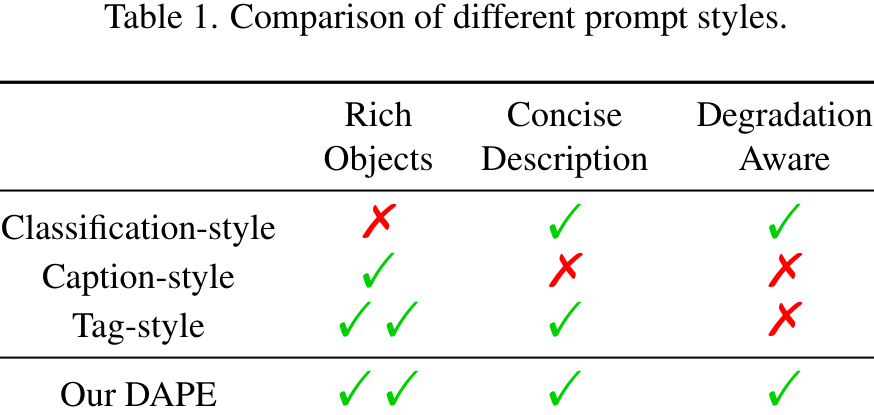
\includegraphics[width=\linewidth]{../original/Table1_p003.png}
\end{tabular}
